\documentclass[fontsize=23pt]{scrreprt}%23pt
\usepackage[a4paper,margin=0.75in,bottom=0.3in,footskip=2em,includefoot]{geometry}%,landscape
\usepackage{amsmath,amsfonts,mathrsfs,amssymb}%,amsthm} 
%\usepackage{pstricks-add}% Pstricks met la page en portrait, bizarrement.
\usepackage{pifont}
\usepackage{yhmath}%pour wideparen
\usepackage{variations}
\usepackage{tabularx}
\usepackage{multicol}
%\usepackage{tikz,tkz-tab}
\usepackage{tikz}
%%%<
\usepackage{verbatim}
%\usepackage[active,tightpage]{preview}
%\PreviewEnvironment{tikzpicture}
\usetikzlibrary{arrows,automata,decorations.markings,calc}
\usepgflibrary{shapes,fpu}
\usepackage{calc}
\usepackage{pifont}
%\usepackage[english]{babel}
\renewcommand{\thesection}{\Roman{section}}
\renewcommand{\labelenumi}{{\textbf{\arabic{enumi}})}}
\renewcommand{\labelenumii}{{\textbf{\alph{enumii}}.}} %--
\renewcommand{\leq}{\leqslant}
\renewcommand{\geq}{\geqslant}
\newcommand{\covec}{\binom}
%EXOS
\newcounter{exercice}
\newcommand{\exo}[1]{% Titre
                     \refstepcounter{exercice}
                     \vspace{1em} \par \noindent
                     \raisebox{-0.7ex}{\textbf{Exercice \no \arabic{exercice}}}
                     \hrulefill\raisebox{-0.7ex}{ \textbf{#1}}
                     \par  \vspace{0.3em} \noindent%
                   }

\usepackage[frenchb]{babel}
\usepackage{pocketmod}
%\usepackage{minilivret}

\usepackage[utf8]{inputenc}
\usepackage[T1]{fontenc}
\usepackage[lining,tabular]{fbb} 
\usepackage[scaled=.95,type1]{cabin} 
%\usepackage[libertine,bigdelims]{newtxmath}
%%
\newcommand{\arc}[1]{\stackrel{\Large \frown}{#1}}
\newcommand{\vv}[1]{\overrightarrow{#1}}
\newcommand{\V}[1]{\overrightarrow{#1}}
\newcommand{\Vu}{\vec{u}}
\newcommand{\Vv}{\vec{v}}
\newcommand{\PS}[2]{\ensuremath{\overrightarrow{#1}\cdot\overrightarrow{#2}}}
\newcommand{\PSuv}[2]{\ensuremath{\vec{u}\cdot\vec{v}}}
\newcommand{\PSvu}[2]{\ensuremath{\vec{u}\cdot\vec{v}}}
%\usepackage{lipsum}
%\usepackage[math]{blindtext}

\title{Trigonométrie}%Anti-sèche \\ *** \\ 
\author{\small Vincent Pantaloni}
\date{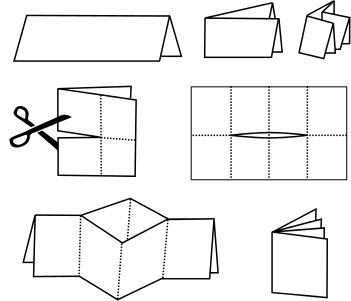
\includegraphics[width=.75\textwidth]{folding-minibook}}
%\date{Lycée Jean Zay}
\setlength{\parindent}{0pt}
%%%%%%%%%%%%%%%%%%%%%%%%%%%%

%%%%%%%%%%%%%%%%%%
\begin{document}
\maketitle
%---------------
\section{Le radian.}
\paragraph{Définition:}   Le \emph{radian} est, comme le degré ou le grade, une unité de mesure d'angles définie de la façon suivante :\\
\begin{minipage}{0.5\textwidth}

   Si l'arc $\wideparen{MN}$ d'un cerle de rayon $R$ a pour longueur $R$, alors l'angle $\widehat{MON}$ vaut $1$ radian. 
 
\end{minipage}\hfill
\begin{minipage}{0.48\textwidth}
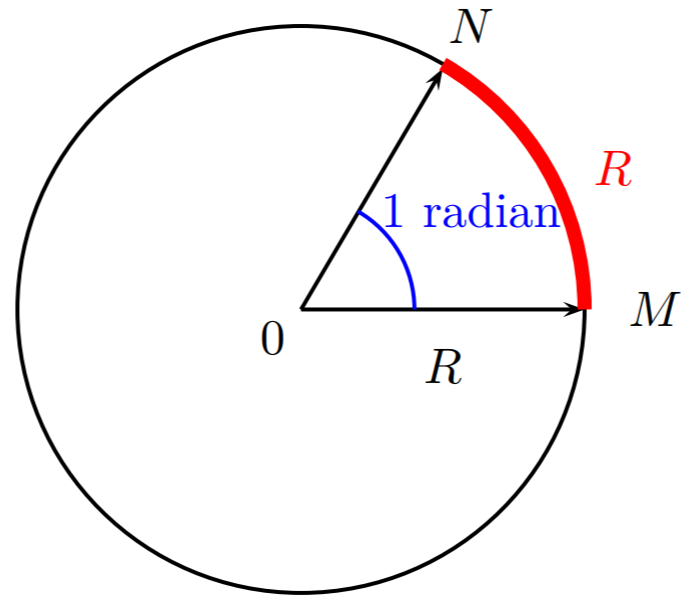
\includegraphics[width=\linewidth]{trigo1}
\end{minipage}
%\\ $360$ degrés $\leftrightarrow 2\pi$ radians.% ou encore $180$ degrés $\leftrightarrow \pi$ radians.
\bigskip

\textit{Remarque:}   La mesure en degrés celle en radians sont proportionnelles: $360$ degrés $\leftrightarrow 2\pi$ radians.

 \noindent \renewcommand{\arraystretch}{2}%   
\begin{center}
\begin{tabular}{|c|*9{c|}}
         \hline 
         Degrés & $360$ &$180$& $120$ & $90$ & $60$ & \phantom{$xx$} & $30$ & &\\ 
         \hline 
         Radians & $2\pi$ &\phantom{$\sum_.^{1}$}  & \phantom{$xx$} &\phantom{$xx$}  & &$\dfrac{\pi}{4}$ & \phantom{$xx$} & $\dfrac{7\pi}{4}$& $\dfrac{11\pi}{12}$\\ 
         \hline 
      \end{tabular} 
      \end{center} 
      %
\paragraph{Définition:} Le \emph{cercle trigonométrique} est le cercle $(\mathscr{C})$ de
        centre $O$, de rayon $1$ muni d'un sens de rotation,
        \emph{i.e.} orienté de telle sorte que le sens positif (ou direct, ou trigonométrique) est celui du sens inverse de rotation des aiguilles d'une montre.
    %
    \newpage
On enroule la droite des réels sur le cercle trigonométrique, dans le sens positif mais aussi dans le sens négatif.


\textbf{Ainsi tout nombre réel $x$ correspond à un point M du cercle.} 

Placer des mesures positives puis négatives en radian sur le cercle trigonométrique:\\[0.5cm]
%\newpage
%\begin{center}

\phantom{.}\hfill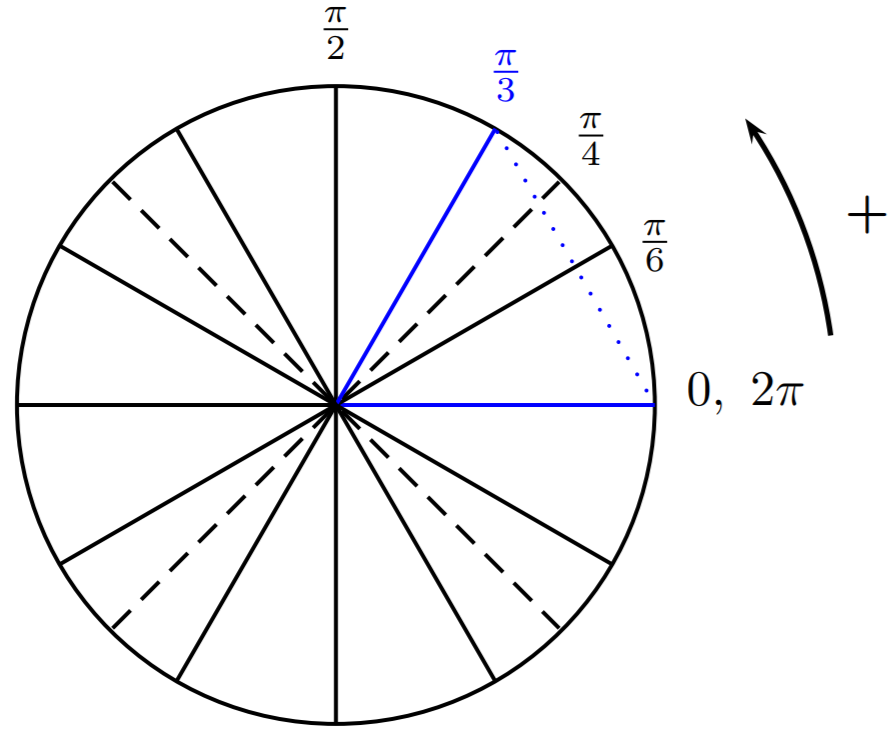
\includegraphics[width=.9\textwidth]{trigo2}
%\end{center}

\newpage
\section{Fonctions sinus et cosinus}%____________________________

%\subsection{Défintions}%____________________________
%\noindent\begin{minipage}{\textwidth - 7cm}
\paragraph{Définition:} 
   Soit $x$ un réel quelconque. Il lui correspond un unique point $M$ de $\mathscr{C}$.
On appelle \emph{cosinus} de $x$, noté $\cos x$ et \emph{sinus} de $x$, noté $\sin x$, les coordonnées du point $M$ dans le repère $(O;\vec{\imath},\vec{\jmath}\,) $.
% tel que $x$ soit une mesure en radians de $(\widehat{\V{OA}, \V{OM}})$
   
\begin{center}
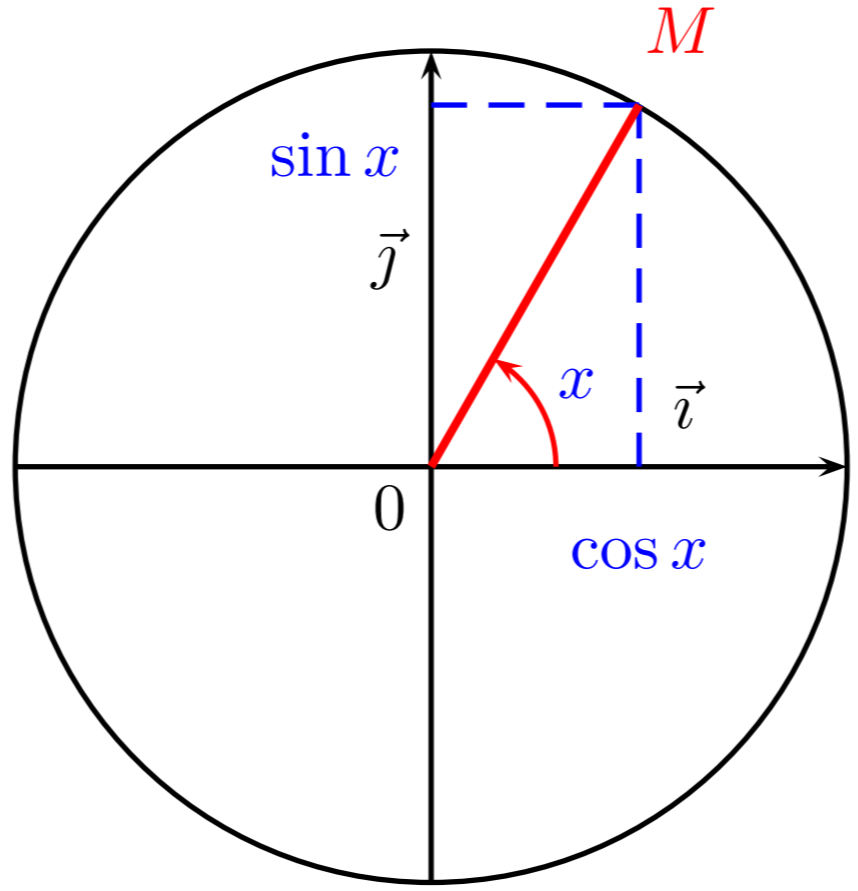
\includegraphics[width=.75\textwidth]{trigo3}
\end{center}

D'après le cercle trigonométrique, on a les prop.:
%\begin{large}

\begin{dingautolist}{168}
      \item $\cos^{2}x + \sin^{2}x=\dots{}\qquad$ (Pythagore)
      \item $\dots{} \leqslant \cos x \leqslant \dots{}$ \quad et \quad $\dots{} \leqslant \sin x \leqslant \dots{}$
      \item $\cos(x+2\pi)=\cos x$  et  $\sin(x+2\pi)=\sin x$
   \end{dingautolist}
 
%\end{large}  
%%%
\subsection*{Variations de cos et sin} %____________________________
%\noindent\begin{minipage}{\textwidth - 7cm}
Par lecture sur le cercle trigonométrique, compléter les deux tableaux de variation et identifier les courbes ci-dessous.

\begin{center}
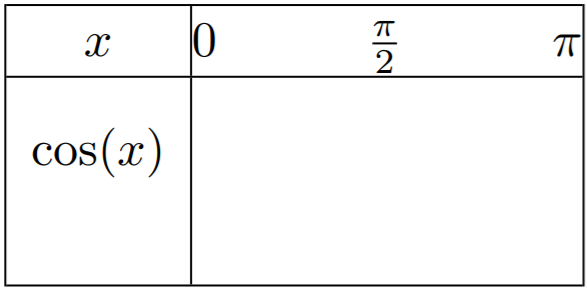
\includegraphics[width=.75\textwidth]{trigo5cos}
\end{center}
\begin{center}
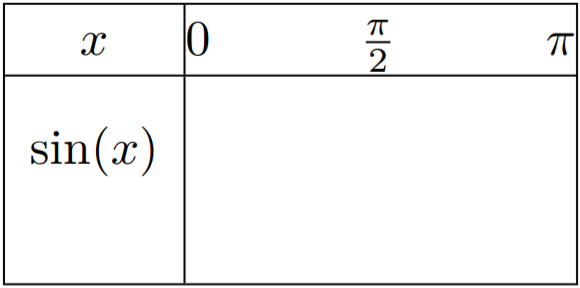
\includegraphics[width=.75\textwidth]{trigo5sin}
\end{center}
\begin{center}
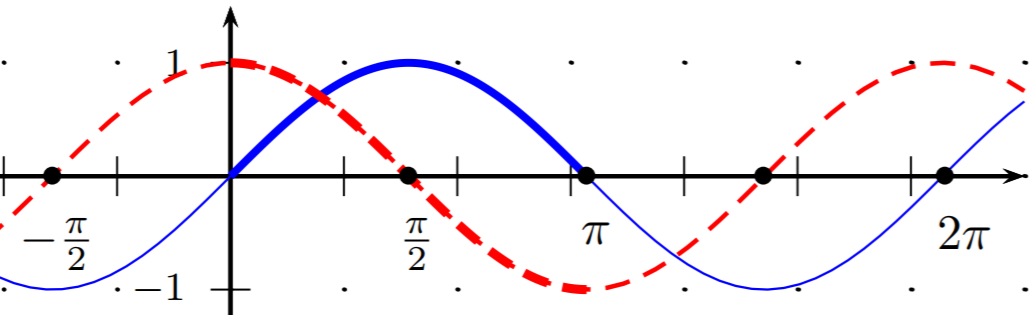
\includegraphics[width=.98\textwidth]{trigo6courbe}
\end{center}
\newpage
\subsection*{Valeurs remarquables}
On retiendra les valeurs remarquables de sin et cos %: \[\dfrac{1}{2},\ \dfrac{\sqrt2}{2},\ \dfrac{\sqrt3}{2}\]
à l'aide du quart de cercle ci-dessous en remarquant que $1<2<3$ donc $1<\sqrt2<\sqrt3$ et donc: 
\[\dfrac{1}{2}< \dfrac{\sqrt2}{2}< \dfrac{\sqrt3}{2}.\]
\begin{center}
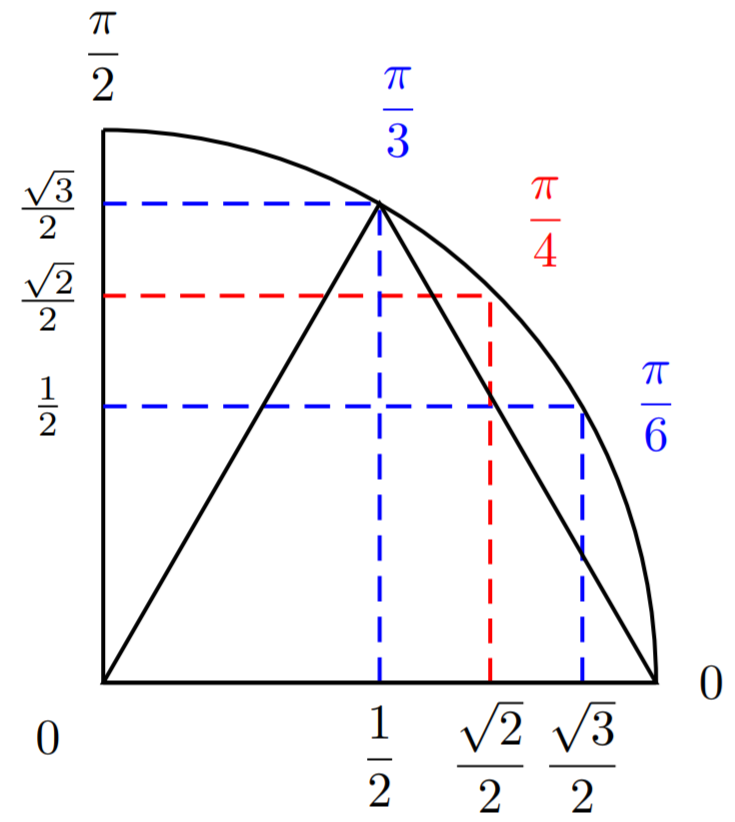
\includegraphics[width=.85\textwidth]{trigo4}
\end{center}
   
%\begin{center}
%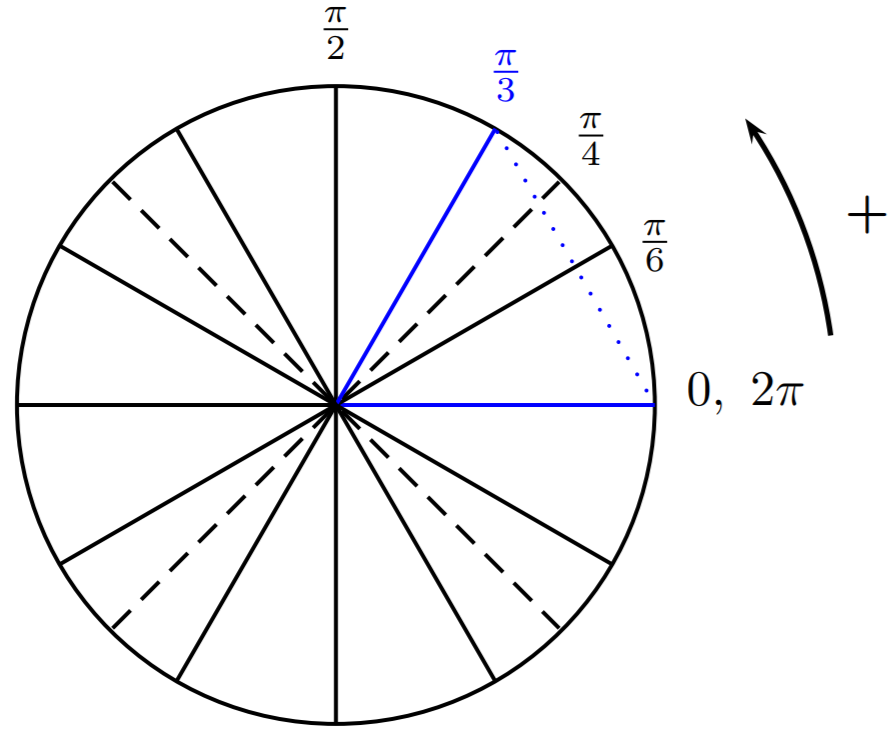
\includegraphics[width=.92\textwidth]{trigo2}
%\end{center}
%

%\newpage
%\rule{0pt}{1cm}
\newpage
%\exo{}
\paragraph{Exercice.} En utilisant les valeurs  remarquables de cos et sin ainsi que des symétries, déterminer les  valeurs exactes demandées.

\begin{enumerate}
\item  $\cos\left(\dfrac{\pi}{4}\right)=\dfrac{\sqrt2}{2}\ $ donc $\cos\left(-\dfrac{\pi}{4}\right)=\dots$
\item  $\cos\left(\dfrac{\pi}{3}\right)=\dfrac12\ $ donc $\cos\left(\dfrac{2\pi}{3}\right)=\dots$
\item  $\sin\left(\dfrac{\pi}{3}\right)=\dfrac{\sqrt3}{2}\ $ donc $\sin\left(\dfrac{2\pi}{3}\right)=\dots$
\item  $\sin\left(\dfrac{\pi}{6}\right)=\dfrac{1}{2}\ $ donc $\sin\left(\dfrac{7\pi}{6}\right)=\dots$

\item  $\sin\left(\dfrac{-\pi}{6}\right)=\dots\ $ et  $\cos\left(-\dfrac{5\pi}{6}\right)=\dots $
\end{enumerate}
\paragraph{Exercice.} \textbf{1)} Sachant qu'un angle $x$ (en radians) est dans $[0;\dfrac{\pi}{2}]$ et que  $\sin(x)=\dfrac{4}{5}$, déterminer  $\cos(x)$. \\
\textbf{2)} On sait que $x\in [0;2\pi]$, et $\cos(x)=-\dfrac{12}{13}$. \\
Quelles sont les valeurs possibles pour  $\sin(x)$? \\[0.5ex]
\textbf{3)} Déterminer les réels $x$ tels que:\\ 
$x\in [0;2\pi]$ et $\cos x=\sin x$.\\[0.5ex]
\textbf{4)} Déterminer les réels $x$ tels que:\\ 
$x\in [-\pi;\pi]$ et $\cos x\geq \dfrac{1}{2}$.
\newpage
\rule{0pt}{3cm}
\begin{center}
\begin{tikzpicture}[scale=7,cap=round,>=latex]%5.3
        % draw the coordinates
        \draw[->] (-1.1cm,0cm) -- (1.1cm,0cm) node[right,fill=white] {$x$};
        \draw[->] (0cm,-1.1cm) -- (0cm,1.1cm) node[above,fill=white] {$y$};

        % draw the unit circle
        \draw[thick] (0cm,0cm) circle(1cm);

        \foreach \x in {0,30,...,360} {
                % lines from center to point
                \draw[gray] (0cm,0cm) -- (\x:1cm);
                % dots at each point
                \filldraw[black] (\x:1cm) circle(0.4pt);
                % draw each angle in degrees
                \draw (\x:0.6cm) node[fill=white] {$\x^\circ$};
        }

        % draw each angle in radians
        \foreach \x/\xtext in {
            30/\dfrac{\pi}{6},
            45/\dfrac{\pi}{4},
            60/\dfrac{\pi}{3},
            90/\dfrac{\pi}{2},
            120/\dfrac{2\pi}{3},
            135/\dfrac{3\pi}{4},
            150/\dfrac{5\pi}{6},
            180/\pi,
            210/\dfrac{7\pi}{6},
            225/\dfrac{5\pi}{4},
            240/\dfrac{4\pi}{3},
            270/\dfrac{3\pi}{2},
            300/\dfrac{5\pi}{3},
            315/\dfrac{7\pi}{4},
            330/\dfrac{11\pi}{6},
            360/2\pi}
                \draw (\x:1.2cm) node[fill=white] {$\xtext$};
                %\draw (\x:0.85cm) node[fill=white] {$\xtext$};

%         \foreach \x/\xtext/\y in {
%             % the coordinates for the first quadrant
%             30/\frac{\sqrt{3}}{2}/\frac{1}{2},
%             45/\frac{\sqrt{2}}{2}/\frac{\sqrt{2}}{2},
%             60/\frac{1}{2}/\frac{\sqrt{3}}{2},
%             % the coordinates for the second quadrant
%             150/-\frac{\sqrt{3}}{2}/\frac{1}{2},
%             135/-\frac{\sqrt{2}}{2}/\frac{\sqrt{2}}{2},
%             120/-\frac{1}{2}/\frac{\sqrt{3}}{2},
%             % the coordinates for the third quadrant
%             210/-\frac{\sqrt{3}}{2}/-\frac{1}{2},
%             225/-\frac{\sqrt{2}}{2}/-\frac{\sqrt{2}}{2},
%             240/-\frac{1}{2}/-\frac{\sqrt{3}}{2},
%             % the coordinates for the fourth quadrant
%             330/\frac{\sqrt{3}}{2}/-\frac{1}{2},
%             315/\frac{\sqrt{2}}{2}/-\frac{\sqrt{2}}{2},
%             300/\frac{1}{2}/-\frac{\sqrt{3}}{2}}
%             \draw (\x:1.25cm) node[fill=white] {$\left(\xtext,\y\right)$};

        % draw the horizontal and vertical coordinates
        % the placement is better this way
%         \draw (-1.25cm,0cm) node[above=1pt] {$(-1,0)$}
%               (1.25cm,0cm)  node[above=1pt] {$(1,0)$}
%               (0cm,-1.25cm) node[fill=white] {$(0,-1)$}
%               (0cm,1.25cm)  node[fill=white] {$(0,1)$};
    \end{tikzpicture}
\end{center}
\end{document}
